The most dominant dynamics of a refridgeration container/trailer are thermal dynamics of the metal in heat exchangers (i.e. evaporator and condensor). Some components in the system will have dynamics so much faster than the dominant dynamics that they will be considered static (compressor and expansion valves).
In the end the model will be composed of a model that represents the refridgeration cycle along with a model of the thermal masses (in heat exchangers, other metal parts and cargo)


\subsection{Component models}

\subsubsection{General type refrigerant control volume state eq}
Many of the components in a refridgeration cycle will be based on similar state equations. They will generally express the change in mass inside the control volume and/or the specific enthalpy out of the control volume. These can be constructed from the mass conservation equation and the energy balance equation of the control volume.

\textbf{Mass conservation equation} \\
\begin{equation} \label{eq:GeneralTypeControlVol_MassConservation}
	\frac{dM}{dt} = \dot{m_{in}} - \dot{m_{out}}
\end{equation}

where 
\begin{center}
	\begin{tabular}{l p{8cm} l}
		$\frac{dM}{dt}$ 	& Change in mass inside control volume & [\si{kg}/\si{s}]\\ 
		$\dot{m_{in}}$ 		& Flow into control volume & [\si{kg}/\si{s}]\\
		$\dot{m_{out}}$ 	& Flow out of control volume & [\si{kg}/\si{s}]\\
	\end{tabular}
\end{center}

\textbf{Energy balance equation}
\begin{equation}
	h_{out} = h_{in} + \frac{Q_{in}}{\dot{m}_{in}}
\end{equation}

where
\begin{center}
	\begin{tabular}{l p{8cm} l}
		$h_{out}$ 		& Specific enthalpy out of the control volume & [\si{J}/\si{kg}]\\ 
		$h_{in}$ 		& Specific enthalpy into control volume & [\si{J}/\si{kg}]\\ 
		$Q_{in}$ 		& Energy flow applied to control volume& [\si{W}]\\
		$\dot{m}_{in}$ 	& Flow into control volume & [\si{kg}/\si{s}]\\
	\end{tabular}
\end{center}

\subsubsection{Expansion valve}
The flow through an expansion valve is proportional to the square root of the pressure drop across it, where the proportional constants relies on physical properties of the valve and refrigerant.
\begin{equation} \label{eq:ExpansionValve}
	\dot{m}= C A \sqrt{\rho\Delta p}
\end{equation}

where 
\begin{center}
	\begin{tabular}{l p{8cm} l}
		$\dot{m}$ 	& Flow through valve & [\si{kg}/\si{s}]\\ 
		$\Delta p$ 	& Pressure drop across valve & [\si{Pa}]\\
		$C$ 		& Discharge coefficient of valve & [$\cdot$]\\
		$A$	 		& Cross sectional area of valve & [\si{m^2}]\\
		$\rho$ 		& Density of liquid & [\si{kg}/\si{m^3}]\\
			$C$ 	& Discharge coefficient of valve & [$\cdot$]\\
	\end{tabular}
\end{center}

To model the way that the valve is intended to be controlled, an alternative representation is introduced for the mass flow through an expansion valve \cref{eq:ExpansionValve_DutyCycle}

\begin{equation} \label{eq:ExpansionValve_DutyCycle}
	\dot{m}= D_{on} K  \sqrt{\frac{1}{v_{in} (p_{in} - p_{out})}}
\end{equation}

where 
\begin{center}
	\begin{tabular}{l p{8cm} l}
		$\dot{m}$	& Flow through valve & [\si{kg}/\si{s}]\\ 
		$D_{on}$ 	& Fraction of each pulse period being on & [$\%$]\\
		$p_{in}$ 	& Absolute pressure on input side & [\si{Pa}]\\
		$K$ 		& $C A$ & [\si{m^2}]\\
		$v_{in}$ 	& Specific volume of liquid & [\si{m^3}/\si{kg}]\\
		$p_{out}$ 	& Absolute pressure on output side & [\si{Pa}]\\
	\end{tabular}
\end{center}

\subsubsection{Pipe Joining Junction} 
Between compressor $ C_1 $, $ C_2 $ and the economizer (see \cref{fig:HVAC_Diagram}) is a Pipe Joining Junction that connects the three forementioned components.

\begin{equation} \label{eq:PipeJoiningJunction_ChangeOfMass}
	\frac{dM}{dt} = \dot{m}_{in1} + \dot{m}_{in2} + \dot{m}_{out}
\end{equation}

where 

\begin{center}
	\begin{tabular}{l p{8cm} l}
		$\frac{dM}{dt}$ & Change in mass inside Pipe Joining Junction		 	& [\si{kg}/\si{s}]\\ 
		$\dot{m}_{in1}$ & Flow into Pipe Joining Junction from Compressor $ C_1 $ 		& [\si{kg}/\si{s}]\\
		$\dot{m}_{in2}$ & Flow into Pipe Joining Junction from Economiser 				& [\si{kg}/\si{s}]\\
		$\dot{m_{out}}$ & Flow into Compressor $ C_2 $ from Pipe Joining Junction		& [\si{kg}/\si{s}]\\
	\end{tabular}
\end{center}

In \cref{eq:PipeJoiningJunction_ChangeOfMass}, the change of mass inside the Pipe Joining Junction can be expressed as a function of the mass flows into and out of the Pipe Joining Junction. 

\begin{equation} \label{eq:PipeJoiningJunction_Enthalpy}
	h_{out} = \frac{h_{in1} \cdot \dot{m}_{in1} + h_{in2} \cdot \dot{m}_{in2}}{ \dot{m}_{in1} + \dot{m}_{in2} }
\end{equation}

where

\begin{center}
	\begin{tabular}{l p{10cm} l}
		$h_{out}$ 	& Specific enthalpy into Compressor $ C_2 $ from Pipe Joining Junction 		& [\si{J}/\si{kg}]\\ 
		$h_{in1}$ 	& Specific enthalpy into Pipe Joining Junction from Compressor $ C_1 $  		& [\si{J}/\si{kg}]\\ 
		$h_{in2}$ 	& Specific enthalpy into Pipe Joining Junction from Economiser   			& [\si{J}/\si{kg}]\\ 
		$\dot{m}_{in1}$ & Flow into Pipe Joining Junction from Compressor $ C_1 $ 		& [\si{kg}/\si{s}]\\
		$\dot{m}_{in2}$ & Flow into Pipe Joining Junction from Economiser 				& [\si{kg}/\si{s}]\\
	\end{tabular}
\end{center}
In \cref{eq:PipeJoiningJunction_Enthalpy} the specific enthalpy of the flow out of the Pipe Joining Junction is expressed as a function of the input flows and enthalpies. This equation is based on the energy balance, assuming no heat transfer to surroundings, i.e. the Pipe Joining Junction is perfectly insulated.

\subsubsection{Pipe Splitting Junction}

This component is particularly simple, as the only function of it is to split the input flow in two. It is furthermore assumed that the dynamics are fast enough that the they can be modelled as algebraic equations.

\begin{equation} \label{eq:PipeSplittingJunction_Enthalpy}
	\begin{split}
		\dot{m}_{in} &= \dot{m}_{out1} + \dot{m}_{out2} \\
		p_{out1} &= p_{in} \\
		p_{out2} &= p_{in} \\
		h_{out1} &= h_{in} \\
		h_{out1} &= h_{in} \\
	\end{split}
\end{equation}

where

\begin{center}
	\begin{tabular}{l p{12cm} l}
		$\dot{m}_{in}$ 		& Mass flow into Pipe Splitting Junction from Condenser (reciever?) 						& [\si{kg}/\si{s}]\\
		$\dot{m}_{out1}$ 	& Mass flow into Economiser expansion valve from Pipe Splitting Junction 				& [\si{kg}/\si{s}]\\
		$\dot{m}_{out2}$ 	& Mass flow into Economiser heat exchanger from Pipe Splitting Junction 					& [\si{kg}/\si{s}]\\
		$p_{in}$ 			& Absolute pressure input Pipe Splitting Junction from Condenser (reciever?)		& [\si{Pa}]\\
		$p_{out1}$ 			& Absolute pressure into Economiser expansion valve from Pipe Splitting Junction 	& [\si{Pa}]\\
		$p_{out2}$ 			& Absolute pressure into Economiser heat exchanger from Pipe Splitting Junction 	& [\si{Pa}]\\
		$h_{in}$ 			& Specific enthalpy into Pipe Splitting Junction from Condenser (reciever?)   		& [\si{J}/\si{kg}]\\ 
		$h_{out1}$ 			& Specific enthalpy into Economiser expansion valve from Pipe Splitting Junction	& [\si{J}/\si{kg}]\\ 
		$h_{out2}$ 			& Specific enthalpy into Economiser heat exchanger from Pipe Splitting Junction		& [\si{J}/\si{kg}]\\ 
	\end{tabular}
\end{center}


The pressure and specific enthalpy on the output flows are equal to the input pressure and specific enthalpy. The sum of the mass flows out of the Pipe Splitting Junction is equal to the input mass flow. \\

\subsubsection{Compressor}
The compressor in the refrigeration cycle consists of two compressor stages that can be described by the same equations.
The compressor dynamics are assumed to be fast enough compared with the refridgeration cycle that it can be considered constant. Therefore, the equations governing the compressors are algebraic equations. 
Adiabatic compression is assumed. 
The two equations describing the compression governs the mass flow and the output specific enthalpy. The output specific enthalpy is found via a lookup table (HTP). 

\begin{align}
	\dot{m} &= \left(\frac{V_1}{v_1} - \frac{V_C}{v_2}\right) \frac{\omega}{2} \\
	h_{out} &= HTP(T_{out}, p_{out}) 
\end{align}

where

\begin{center}
	\begin{tabular}{l p{8cm} l}
		$\dot{m}$				& Flow through compressor stage					& [\si{kg}/\si{s}]\\ 
		$h_{out}$				& Compressor stage output specific enthalpy				& [\si{J}/\si{kg}]\\ 
		$V_1$					& Cylinder internal volume b.f. stroke			& [$\si{m}^3$]\\ 
		$V_C$					& Cylinder clearance volume after stroke		& [$\si{m}^3$]\\ 
		$v_1$					& Refrigerant specific volume b.f. stroke		& [$\si{m}^3/\si{kg}$]\\
		$v_2$					& Refrigerant specific volume after stroke		& [$\si{m}^3/\si{kg}$]\\
		$\omega$ 				& Compressor angular velocity 					& [\si{rad}/\si{s}]\\
		$T_{out}$ 				& Compressor stage output temperature 			& [\si{K}]\\
		$p_{out}$				& Compressor stage output pressure 				& [\si{Pa}]\\
	\end{tabular}
\end{center}

\begin{align}
	v_2 &= \left(\frac{p_2}{p_1}\right)^{\frac{-1}{\gamma}} \\
	p_1 &= p_{in} - kl_1 \cdot \omega \\
	p_2 &= p_{out} + kl_2 \cdot \omega \\
	\gamma &= C_{cp}/C_{cv} \\
	T_{out} &= T_{in}\cdot \left(\frac{p_{out}}{p_{in}}\right)^{\frac{\gamma-1}{\gamma}}
\end{align}

where 

\begin{center}
	\begin{tabular}{l p{8cm} l}
		$p_{in}$				& Compressor stage input pressure 			& [\si{Pa}]\\
		$p_1$					& Piston input pressure									& [\si{Pa}]\\ 
		$p_2$					& Piston output (discharge) pressure 		& [\si{Pa}]\\ 
		$\gamma$				& Heat capacity ratio 								& [$ \cdot $]\\
		$ kl_1$, $kl_2$			& Valve loss constants							& [$ \cdot $]\\
		$\omega$ 				& Compressor angular velocity 				& [\si{rad}/\si{s}]\\
		$T_{in}$ 				& Compressor stage input temperature 	& [\si{K}]\\
		$C_{cp}$ 				& Specific heat capacity - constant pressure 	& [\si{J}/(\si{kg}\si{K})]\\
		$C_{cv} $ 				& Specific heat capacity - constant volume 	& [\si{J}/(\si{kg}\si{K})]\\
	\end{tabular}
\end{center}

\subsubsection{Condenser}

The condenser takes in the discharge pressure vapor from the second compressor stage, at point 4 in \cref{fig:HVAC_Diagram}. The high pressure also yields a high temperature, 
which enables heat transfer through the condensor to ambient air. This is done mainly through condensation of the refrigerant vapor, yielding high pressure liquid at point 5 in \cref{fig:HVAC_Diagram}.
The energy balance is modelled in \cref{eq:Condenser_Enthalpy}. The mass balance is modelled in \cref{eq:Condenser_ChangeOfMass}. Finally the temperature of the metal in the condenser is modelled in 
\cref{eq:Condenser_ChangeOfTemperature}, as the dominant dynamics of the condenser is greatly linked to the temperature of the metal \cite{Sorensen2013}. \cref{eq:Condenser_ChangeOfTemperature} is also 
derived from the energy balance.

\begin{align}
	h_{out} 			& = h_{in} - \frac{Q_{rm}}{\dot{m}_{in}}  	\label{eq:Condenser_Enthalpy} \\
	\frac{dM_r}{dt} 	& = \dot{m}_{in} - \dot{m}_{out} 				\label{eq:Condenser_ChangeOfMass}\\
	\frac{dT_m}{dt} 	& = \frac{Q_{rm} - Q_{ma}}{M_m \cdot Cp_m}		\label{eq:Condenser_ChangeOfTemperature}
\end{align}

where 

\begin{center}
	\begin{tabular}{l p{8cm} l}
		$h_{out}$				&  Condenser output specific enthalpy			& [\si{J}/\si{kg} ]\\
		$h_{in}$					&  Condenser input specific enthalpy 			& [\si{J}/\si{kg}] \\
		$Q_{rm}$					& Refrigerant to metal heat flow 			& [\si{W}] \\
		$Q_{ma}$					& Metal to air heat flow						& [\si{W}] \\
		$\dot{m_{in}}$			& Condenser input mass flow 			& [\si{kg}/\si{s}] \\
		$\dot{m_{out}}$			& Condenser output mass flow 		& [\si{kg}/\si{s}] \\
		$M_r$						& Refrigerant mass 								& [\si{kg}] \\
		$M_m$						& Metal mass												& [\si{kg}] \\
		$T_m$						& Metal temperature 							& [\si{K}]\\
		$Cp_m$					& Metal heat capacity 						& [\si{J}/\si{K}]\\
		$$				&  			& []

	\end{tabular}
\end{center}

The pressure differential across the condenser is assumed to be linear, yielding \cref{eq:Condenser_PressureDrop}.
The mass flow out of the condenser is modelled in \cref{eq:Condenser_MassFlow}.


\begin{align}
	p_{in}	 			& = p_{out} - \lambda \cdot \dot{m}_{in}  				\label{eq:Condenser_PressureDrop}\\
	\dot{m}_{out}		& = \dot{m}_{in} + \frac{M_r - \frac{V_i}{v}}{ls}		\label{eq:Condenser_MassFlow}
\end{align}

And finally the convective heat flows are modelled in \cref{eq:Condenser_HeatFlow_rm}, \cref{eq:Condenser_HeatFlow_ma}. $ U_{fan}	 $ will have a base value that is non zero ($ \sim $ 0.05) even when the fan is off due to natural convection.

\begin{align}
	Q_{rm}	 			& = U A_{rm} \cdot (T_r - T_m)							\label{eq:Condenser_HeatFlow_rm}\\
	Q_{rm}	 			& = U A_{ma} \cdot (T_m - T_a)\cdot U_{fan}				\label{eq:Condenser_HeatFlow_ma}
\end{align}	

\subsubsection{Flash tank}
The flash tank in combination with the condenser throttle valve serves to reduce the amount of high enthalpy flash gas delivered to the evaporator. The condenser throttle valve, the dynamics of which is identical to the expansion valve, lowers the pressure of the liquid from the condenser. This naturally lowers the temperature, but also generates some amount of flash gas. The flash tank then separates the liquid-vapor mixture and passes only the liquid to the expansion valve. The flash gas is returned to the second stage of the compressor, where it is reused. Thus, a lower amount of flash gas will be generated by the expansion valve, as the pressure of the liquid is already quite low.

The modelling will only evaluate the steady state behaviour of the flash tank. This is due to the tedious nature of the problem and the limited scope of the project. 

In steady state it is first assumed that the pressure of the liquid-vapor mixture entering is the same as the separated liquid and vapor leaving the tank. 
\begin{align}
	p_{lv} 	= p_{l}					&  = p_{v} 
	\label{eq:Flash_tank_pressure} \\
\end{align}

where 

\begin{center}
	\begin{tabular}{l p{8cm} l}
		$p_{lv}$				&  Liquid-vapor mixture pressure		& [\si{Pa}]\\
		$p_{l}$					&  Liquid pressure 						& [\si{Pa}] \\
		$p_{v}$					&  Vapor pressure						& [\si{Pa}]\\
		
	\end{tabular}
\end{center}


Secondly, it is assumed that the energy of the mixture does not change, meaning the energy flow in equals the energy flow out. 
\begin{align}
	\dot{m}_{lv} \cdot  h_{lv}  - \dot{m}_{l} \cdot  h_{l} - \dot{m}_{v} \cdot  h_{v} & = 0
	\label{eq:Flash_tank_energyflow} \\
\end{align}

where 

\begin{center}
	\begin{tabular}{l p{8cm} l}
		$\dot{m}_{lv}$			&  Liquid-vapor mixture mass flow			& [\si{kg}/\si{s}]\\
		$\dot{m}_{l}$			&  Liquid mass flow 						& [\si{kg}/\si{s}] \\
		$\dot{m}_{v}$			&  Vapor mass flow							& [\si{kg}/\si{s}]\\
		$h_{lv}$				&  Liquid-vapor mixture specific enthalpy	& [\si{J}/\si{kg}]\\
		$h_{l}$					&  Liquid specific enthalpy 				& [\si{J}/\si{kg}] \\
		$h_{v}$					&  Vapor specific enthalpy					& [\si{J}/\si{kg}]\\
		
	\end{tabular}
\end{center}


Lastly, it is assumed that the separated liquid and vapor leaves at boiling point and flash point respectively. This last assumption allows us to find the enthalpy of the two substances purely from investigation of the PH diagram and the pressure. In practice, this is performed by a software tool as MATLAB.

\subsubsection{Subcooling throttle}
The subcooling throttle valve is used differently from the two other valves in the system. During normal operation it is fully open, acting as a pipe. It can be closed fully allowing for various speciel functionalities. Firstly, shutting it off allows for detecting the amount of refridgerant in the system. This is a convenient diagnostic feature which helps ensuring that the system has enough refridgerant to properly function, and enabling leakage detection. Secondly, closing the valve while fully opening the condenser throttle valve, allows the system to operate as a standard refridgeration system, with only one valve between the evaporator and condenser.

\subsubsection{Evaporator}
The superheat of the evaporator is an important and difficult state to control. It is important as the compressor can be damaged if the refrigerant contains liquid. Additionally the superheat is important from an efficiency point of view. 
The superheat is the difference between the vapor saturation temperature and the actual temperature at the compressor suction inlet. It is a measure of excess energy transferred to the refrigerant. 

The evaporator is split into two control volumes, divided by a moving CV boundary $\sigma$ which divides liquid-vapor mixture and the superheated vapor.

Because the heat transfer coefficient between liquid and metal and vapor and metal, the metal is likewise split by the $\sigma$ boundary.

The modeling of $\sigma$ is based on an assumption that the refrigerant has a constant average quality throughout the liquid-vapor mixture.

\begin{figure}[h!]
	\centering
	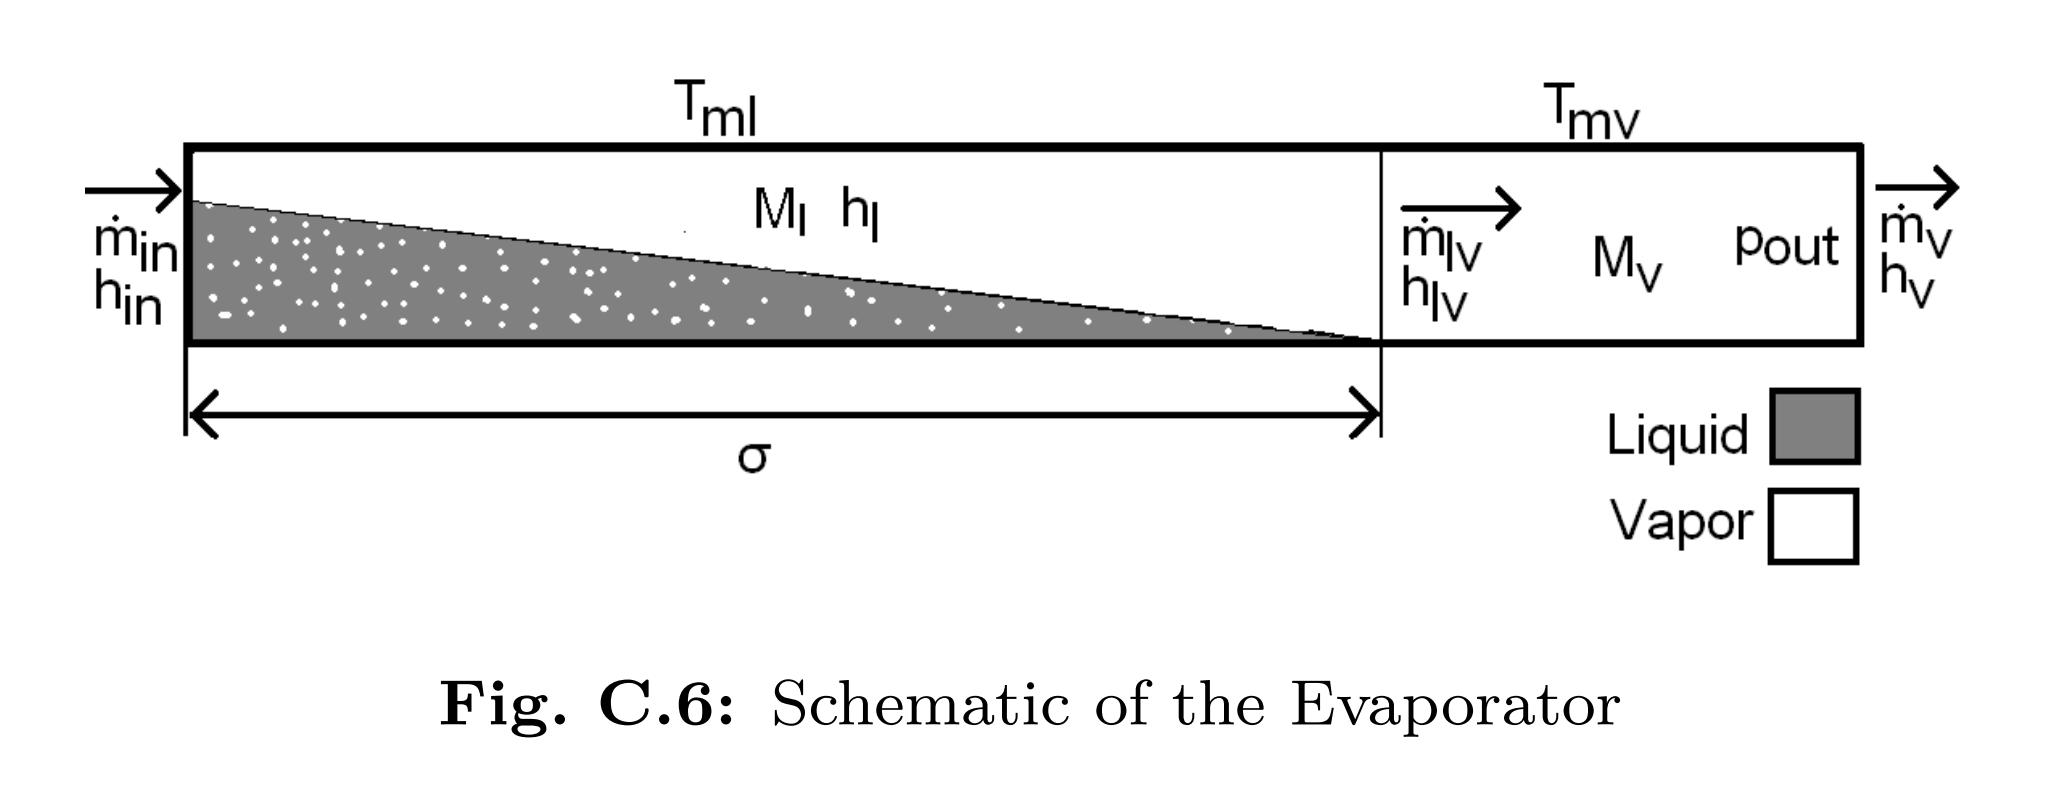
\includegraphics[width=0.6\textwidth]{Graphics/evaporator_CV_stolen.jpeg}
	\caption{Stolen evaporator CV diagram \cite{Sorensen2013}}
	\label{fig:evapo_CV}
\end{figure}






The calculation of the boundary location can be seen in \cref{eq:Evaporator_boundary}
\begin{equation} \label{eq:Evaporator_boundary}
	\sigma = \frac{M_l \cdot v_1}{V_i} 
\end{equation}

where

\begin{center}
	\begin{tabular}{l p{8cm} l}
		$\sigma$				& Control Volume boundary 			& [$\cdot$] \\		
		$M_l$				& Mass of liquid-vapor CV 			& [\si{kg}] \\		
		$v_1$				& Refrigerant specific volume of vapor-liquid CV	& [$\si{m}^3/\si{kg}$] \\		
		$V_i$				& Evaporator volume 			& [$\si{m}^3$]
	\end{tabular}
\end{center}


The heat flows and temperatures relating to the evaporator is modeled by the following equations:
\begin{align}
	Q_{fan} 		& = (155 \cdot U_{fan}^2 + 40 \cdot U_{fan}^3) \cdot 0.2 \\
	T_{retfan} 		& = T_{ret} + \frac{Q_{fan}}{\dot{m}_{air} \cdot Cp_{air}} \\
	Q_{amv} 		& = Cp_{air} \cdot \dot{m}_{air} \cdot (T_{retfan} - T_{mv}) \\
	T_{retsh} 		& = T_{retfan} - \frac{Q_{amv}}{\dot{m}_{air} \dot Cp_{air}} \\
	Q_{aml} 		& = Cp_{air} \cdot \dot{m}_{air} \cdot (T_{retsh} - T_{ml}) \\
	Q_{mvml} 		& = U A_3 \cdot (T_{mv} - T_{ml}) \\
	Q_{ml} 			& = U A_1 \cdot (T_{ml} - T_l) \cdot \sigma\\
	Q_{mv} 			& = U A_2 \cdot (T_{mv} - T_v) \cdot (1- \sigma)
\end{align}

where

\begin{center}
	\begin{tabular}{l p{10cm} l}
		$Q_{fan}$			& Heat added from fan to air (heatloss)			& [\si{W}] \\	
		$Q_{aml}$			& Heat flow from air to metal surrounding liquid-vapor CV			& [\si{W}] \\	
		$Q_{amv}$			& Heat flow from air to metal surrounding vapor CV			& [\si{W}] \\		
		$Q_{mvml}$			& Heat flow from through from metal surrounding vapor CV to metal surrounding liquid-vapor CV			& [\si{W}] \\	
		$Q_{ml}$			& Heat flow from evaporator metal to liquid-vapor CV			& [\si{W}] \\	
		$Q_{mv}$			& Heat flow from evaporator metal to vapor CV					& [\si{W}] \\			
		$U_{fan}$			& Fan speed 	& [rad/s ???? ]\\
		$T_{ret}$			& Return temperature of air coming from trailer 			& [\si{K}] \\		
		$T_{retfan}$		& Temperature of return air after passing through fan			& [\si{K}] \\		
		$T_{mv}$			& Temperature of metal on the vapor CV			& [\si{K}] \\
		$T_{ml}$			& Temperature of metal on the liquid-vapor CV			& [\si{K}] \\
		$T_{retsh}$			& Temperature of air over superheated vapor CV			& [\si{K}] \\
		$T_{l}$				& Saturation temperature for evaporation of the refrigerant			& [\si{K}] \\	
		$T_{v}$				& Temperature of refrigerant (vapor) leaving the evaporator		& [\si{K}] \\		
		$\dot{m}_{air}$		& Mass flow of air through fan			& [\si{kg}/\si{s}] \\		
		$Cp_{air}$			& Specific heat capacity of air			& [\si{J}/(\si{K}\si{kg})] \\	
		$UA_1$				& Heat transfer coefficient from metal to liquid			& [\si{J}/\si{K}] \\
		$UA_2$				& Heat transfer coefficient from metal to vapor			& [\si{J}/\si{K}] \\
		$UA_3$				& Heat transfer coefficient from metal surrounding vapor CV to metal surrounding liquid-vapor CV			& [\si{J}/\si{K}] \\
	\end{tabular}
\end{center}

The airflow over the evaporator is dynamic in itself, as the airflow is driven by a fan that has rotational inertia. Additionally, as the air is a fluid by itself, it contains some inetia too. This behaviour is modeled by:

\begin{align}
	\bar{\dot{m_{air}}} & = \frac{U_{fan}^2 \cdot 3400.5 + U_{fan}^3 \cdot -1103.5} {3600 \cdot \rho_{air}} \label{eq:Evaporator_FanAirInstantMassFlow}\\ 
	\frac{\Delta \dot{m_{air}}}{\Delta t} & = \frac{\bar{\dot{m_{air}}} - \dot{m_{air}}} {10s} \label{eq:Evaporator_FanAirRateOfChange}
\end{align} \todo{Does this still hold for a variable frequency Fan drive? If not, maybe we can start out with it modelled statically or without it?}

where

\begin{center}
	\begin{tabular}{l p{8cm} l}
		$\bar{\dot{m}}_{air}$						& Instant steady state estimate mass flow of air  		& [\si{kg}/\si{s}] \\		
		$\dot{m}_{air}$								& Actual mass flow of air								& [\si{kg}/\si{s}] \\		
		$U_{fan}$									& Fan speed 											& [rad/s ????] \\		
		$\rho_{air}$								& Density of air										& [\si{kg}/\si{m^3}] \\[0.2cm]		
		$\dfrac{\Delta \dot{m}_{air}}{\Delta t} $ 	& The rate of change of	air flow 						& [\si{kg}/\si{s^2}]
	\end{tabular}
\end{center}

\cref{eq:Evaporator_FanAirInstantMassFlow} calculates the steady state air mass flow at new speed. \cref{eq:Evaporator_FanAirRateOfChange} approximates the rate of change of the air mass flow as a first-order difference with time constant of 10 seconds. \\

The remaining state equations are given by equations:

\begin{align}
	\frac{dT_{ml}}{dt} & = \frac{Q_{aml}-Q_{ml} + Q_{mvml}}{M_m \cdot Cp_m \cdot \sigma} \\
	\frac{dT_{mv}}{dt} & = \frac{Q_{amv} - Q_{mv} - Q_{mvml}}{M_m \cdot Cp_m \cdot (1- \sigma)} \\
	p_{out} & = PHV \left( h_v, \frac{V_i-V_l}{M_v} \right)\\
	h_l & = h_{in} + \frac{Q_{ml}}{\dot{m_{in}}}\\
	h_v & = h_{lv} + \frac{Q_{mv}}{\dot{m_{lv}}}\\
	\frac{dM_l}{dt} & = \dot{m_{in}} - \dot{m_{lv}}\\
	\frac{dM_v}{dt} & = \dot{m_{lv}} - \dot{m_{out}}\\
	T_{sup} & = T_{retfan} +  \frac{Q_{aml} + Q_{amv}}{Cp_{air} \cdot \dot{m_{air}}} \\
	\dot{m_{lv}} & = \frac{Q_{ml}}{h_{dew} - h_{in}}
\end{align}

where\\


\begin{center}
	\begin{tabular}{l p{10cm} l}
		$\dfrac{d T_{ml}}{dt} $		& Change of metal temperature in liquid-vapor CV  			& [\si{K}/\si{s}] \\[0.3cm]		
		$\dfrac{d T_{mv}}{dt} $		& Change of metal temperature in vapor CV					& [\si{K}/\si{s}] \\[0.3cm]		
		$\dfrac{d M_{l}}{dt} $		& Change of mass in	in liquid-vapor CV 						& [\si{kg}/\si{s}] \\[0.3cm]		
		$\dfrac{d M_{v}}{dt} $		& Change of mass in	in vapor CV								& [\si{kg}/\si{s}] \\[0.3cm]		
		$Q_{aml}$					& Heat flow from air to metal surrounding liquid-vapor CV	& [\si{W}] \\	
		$Q_{amv}$					& Heat flow from air to metal surrounding vapor CV			& [\si{W}] \\		
		$Q_{mvml}$					& Heat flow from through from metal surrounding vapor CV to metal surrounding liquid-vapor CV			& [\si{W}] \\	
		$Q_{ml}$					& Heat flow from evaporator metal to liquid-vapor CV		& [\si{W}] \\	
		$Q_{mv}$					& Heat flow from evaporator metal to vapor CV				& [\si{W}] \\				
		$M_{m} $					& Mass of metal												& [\si{kg}] \\	
		$M_{v} $					& Mass of vapor												& [\si{kg}] \\	
		$V_{i} $					& Total volume of evaporator								& [\si{m^3}] \\	
		$V_{l} $					& Volume of liquid refrigerant								& [\si{m^3}] \\	
		$Cp_{air}$					& Specific heat capacity of metal							& [\si{J}/(\si{K}\si{kg})] \\	
		$Cp_{air}$					& Specific heat capacity of air								& [\si{J}/(\si{K}\si{kg})] \\	
		$\sigma$					& Control Volume boundary 									& [$\cdot$] \\		
		$PHV $						& Table lookup of pressure, where inputs are specific enthalpy and density								& [] \\	
		$h_{v} $					& Specific enthalpy of vapor CV								& [\si{J}/\si{kg}] \\	
		$h_{l} $					& Specific enthalpy of liquid-vapor CV						& [\si{J}/\si{kg}] \\	
		$h_{in} $					& Specific enthalpy of input liquid refrigerant 			& [\si{J}/\si{kg}] \\	
		$h_{lv} $					& Specific enthalpy of refrigerant moving from liquid-vapor CV to vapor CV						& [\si{J}/\si{kg}] \\
		$h_{dew}$					& Specific enthalpy of dew point specific enthalpy at evaporator pressure, where liquid refrigerant changes phase to vapor		& [\si{J}/\si{kg}] 		\\	
		$\dot{m}_{in} $				& Mass flow of input refrigerant 							& [\si{kg}/\si{s}] \\	
		$\dot{m}_{lv} $				& Mass flow of refrigerant from liquid-vapor CV to vapor CV	& [\si{kg}/\si{s}] \\	
		$\dot{m}_{out} $			& Mass flow of output refrigerant							& [\si{kg}/\si{s}] \\	
		$\dot{m}_{air}$				& Actual mass flow of air									& [\si{kg}/\si{s}] \\				
		$T_{sup} $					& Temperature of air flowing into trailer					& [\si{K}] \\	
		$T_{retfan}$				& Temperature of return air after passing through fan		& [\si{K}] \\	
		$ p_{out} 	$				& Pressure in evaporator									& [\si{Pa}] \\	
	\end{tabular}
\end{center}


\subsubsection{Box}
The trailer box contains by far the greatest thermodynamic capacities due to the large mass of the aluminum T-floor and cargo. The cargo and T-floor temperatures are strongly coupled to the surrounding air temperature due to their large surface area. The temperatures of the three main thermal capacities are modeled and their state space equations are given as below:

\begin{align}
	\frac{dT_{air}}{dt} & = \frac{Q_{ca} + Q_{aa} + Q_{fa} + Q_{fan} -Q_{cool}}{M_{air} \cdot Cp_{air}} \\
	\frac{dT_{floor}}{dt} & = \frac{Q_{af} - Q_{fa}}{M_{floor} \cdot Cp_{floor}} \\
	\frac{dT_{cargo}}{dt} & = \frac{-Q_{ca}}{M_{cargo} \cdot Cp_{cargo}}
\end{align}

where
\begin{center}
	\begin{tabular}{l p{8cm} l}
		$Q_{ca}$			& Cargo to air heat flow					& [\si{W}] \\		
		$Q_{aa}$			& Ambient (walls and roof) to air heat flow		& [\si{W}] \\		
		$Q_{fa}$			& Floor to air heat flow 						& [\si{W}] \\		
		$Q_{af}$			& Ambient (floor) to floor heat flow 	& [\si{W}] \\		
		$Q_{fan}$			& Fan to air heat flow 						& [\si{W}] \\		
		$Q_{cool}$			& Air to evaporator heat flow  			& [\si{W}] \\		
		$T_{air}$			& Air temperature 								& [\si{K}] \\
		$T_{floor}$			& Floor temperature						& [\si{K}] \\
		$T_{cargo}$		& Cargo temperature							& [\si{K}] \\
		$M_{air}$			& Air mass										& [\si{kg}] \\
		$M_{floor}$			& Floor mass								& [\si{kg}] \\
		$M_{cargo}$		& Cargo mass								& [\si{kg}] \\		
		$Cp_{air}$			& Air heat capacity							& [\si{J}/\si{kg} \si{K}] \\
		$Cp_{floor}$	& Floor heat capacity						& [\si{J}/\si{kg} \si{K}] \\
		$Cp_{cargo}$	& Cargo heat capacity					& [\si{J}/\si{kg} \si{K}]
	\end{tabular}
\end{center}

The heat flows are modeled as

\begin{align}
	Q_{cool} & = Cp_{air} \cdot \dot{m_{air}} \cdot (T_{ret} - T_{sup}) \label{eq:box_Qcool}\\
	Q_{aa} & = (T_{amp} - T_{air}) \cdot U A_{amp} \cdot 0.81 \label{eq:box_hf_wall-to-air} \\
	Q_{af} & = (T_{amp} - T_{floor}) \cdot U A_{amb} \cdot 0.19 \label{eq:box_hf_floor-to-air} \\
	Q_{ca} & = (T_{cargo} - T_{air}) \cdot U A_{cargo}\\
	Q_{fa} & = (T_{floor} - T_{air}) \cdot U A_{floor}\\
	Q_{fan} & = (155 \cdot U_{fan}^2 + 40 \cdot U_{fan}^3) \cdot 0.8
\end{align}

where
\begin{center}
	\begin{tabular}{l p{8cm} l}
		$\dot{m}_{air}$			& Air mass flow 									& [\si{kg}/{\si{s}}] \\		
			$T_{ret}$			& Return air temperature 							& [\si{K}] \\		
			$T_{sup}$			& Supply air temperature							& [\si{K}] \\		
			$T_{amb}$			& Wall and floor temperature 						& [\si{K}] \\		
			$U A_{amb}$			& Wall and floor heat transfer coefficient 			& [\si{W}/\si{K}] \\		
			$U A_{cargo}$		& Cargo heat transfer coefficient 					& [\si{W}/\si{K}] \\		
			$U A_{floor}$		& Floor heat transfer coefficient 					& [\si{W}/\si{K}] \\		
			$U_{fan}$			& Fan Speed 										& [$\cdot$]
	\end{tabular}
\end{center}
	
	$Q_{cool}$ is the cooling provided by the evaporator. It is calculated based on the difference between the temperature of the air reaturning from the box ($T_{ret}$) and the temperature of the air supplied to the box $T_{sup}$ as seen in \cref{eq:box_Qcool}
	
	The heat transfer coefficient of the walls and floor are expected to be given by the cooling trailer manufacturer. In the case of the cooling container a heat transfer coefficient was given ($U A_{amb}$) for both the walls and the floor. In this case the ratio of the floor and walls with regards to the total surface area of the container were multiplied with this coefficient as seen in \cref{eq:box_hf_wall-to-air} and \cref{eq:box_hf_floor-to-air}





\subsubsection{Thermodynamic}

\begin{itemize}
	\item Compressor (static) \cite{Sorensen2013} p. 122
	\item Condensor
	\item Reciever
	\item Valve (static) \cite{Sorensen2013} p. 122
	\item Economizer
	\item Evaporator
	\item Pipe joining junction
	\item Pipe splitting junction
	\item Box
\end{itemize}

\subsubsection{Electric}

\begin{itemize}
	\item Battery
	\item Inverter
\end{itemize}

\subsection{Collection of components}

\subsubsection{Linearisation}